\documentclass[t]{beamer} 
\usepackage{amsmath}
\usepackage{amsthm}
\usepackage[T1]{fontenc}
\usepackage{lmodern}
\usepackage{color}
\usepackage{xcolor}
\usepackage{hyperref}
\usepackage{multirow,varwidth} % used for SL table
\usepackage{tikz}
\usepackage{multicol}
\usepackage{graphicx}
\usepackage{etoolbox}
\usepackage{bm}
\usepackage[abs]{overpic}
\usepackage{pict2e}
\usepackage{animate}
\usepackage{verbatim}
\usepackage{soul}
\usepackage{xmpmulti}
\usepackage{subfig}
\usepackage{media9}


\usetheme{PaloAlto}
\usecolortheme{seahorse}


\newenvironment{withoutheadline}{ 
\setlength{\headheight}{0pt} 
\setbeamertemplate{headline}{}}

\setbeamercolor*{block title example}{fg=white,
bg= black!30!blue}
\setbeamercolor*{block body example}{fg=black,
bg= blue!5}

\setbeamertemplate{frametitle continuation}{}

\setbeamertemplate{footline}{}

\setbeamertemplate{itemize items}[circle]
\setbeamertemplate{navigation symbols}[only frame symbol]
\setbeamerfont{framesubtitle}{size=\large}


\title{{\bf Targeted Learning, HAL, (Deep LTMLE) and Causal Inference for Generating Real World Evidence}}
%\subtitle{Towards integration of Targa future informed by real world evidence}
\author{Mark van der Laan}


\institute{Jiann-Ping Hsu/Karl E. Peace Professor in Biostatistics \& Statistics University of California, Berkeley}

\date{August 7, 2024, JSM 2024, Portland\\
%Introduction to Targeted Learning\\
%\date{September 6-7, ISPOR 2023\\
%Part of Short Course Targeted Learning for Generating Real World Evidence\\

{\tiny \vspace{3pt} Acknowledgements: Maya Petersen, Rachael Phillips, Susan Gruber, Ivana Malenica, Toru Shirakawa; Yi Li, Sky Qiu}
}

\begin{document}

\begin{frame}[noframenumbering]
\titlepage
\end{frame}

%\section{Traditional Statistics}\begin{frame}\frametitle{Traditional toolbox for statistics: Recipe oriented, enforces false constraints, not made for Big Data}\vspace{-12pt}\centering\begin{figure}%\includegraphics[width=.75\textwidth]{statisticsForDummies.png}\includegraphics[width=.73\textwidth]{statistics-for-dummies.png}
% Source: https://www.graphpad.com/support/faqid/1790/\end{figure}\end{frame}\begin{frame}\frametitle{Performance of traditional tools: Coverage of Confidence Intervals deteriorates with sample size}\vspace{5pt}\centering
%Nima graphic n increasing, coverage to 0.\includegraphics[width=\textwidth]{coverage_turing.pdf}\end{frame}\begin{frame}\frametitle{Performance of traditional tools: Type I error deteriorates with sample size}\vspace{5pt}\centering%Nima graphic n increasing, type-1 error to 1.\includegraphics[width=\textwidth]{error_turing.pdf}\end{frame}\begin{frame}\frametitle{Traditional tools invite/encourage post-hoc model manipulation}\centering\vspace{-.11in}\begin{figure}\includegraphics[width=0.62\textwidth]{comic.png}\end{figure}\end{frame}\begin{frame}\frametitle{Why care about statistical inference?}\vspace{-.2in}\centering\begin{figure}\fbox{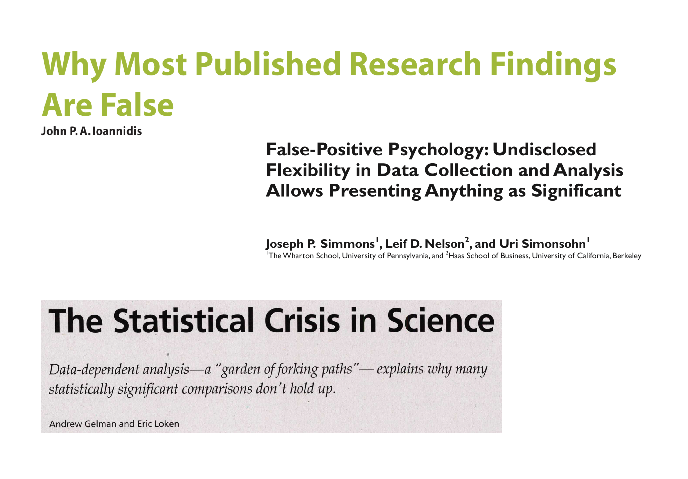
\includegraphics[width=.99\textwidth]{articles.pdf}}\end{figure}\end{frame}

%\begin{frame}
%\frametitle{Expectations vs. Reality: What are we actually estimating?}
%\centering
%\begin{figure}
%\includegraphics[width=1.03\textwidth]{538graphic.png}
%\end{figure}
%\end{frame}

%The challenge facing modern statisticians (and you, as students in this %class) is how to develop statistical methods aimed at answering specific %scientific questions of interest, while utilizing state-of-the-art %algorithms.

%\section{Overview TL}

%\begin{frame}\frametitle{Targeted Learning for answering statistical and causal questions with confidence intervals} \vspace{-1em}  \begin{center}  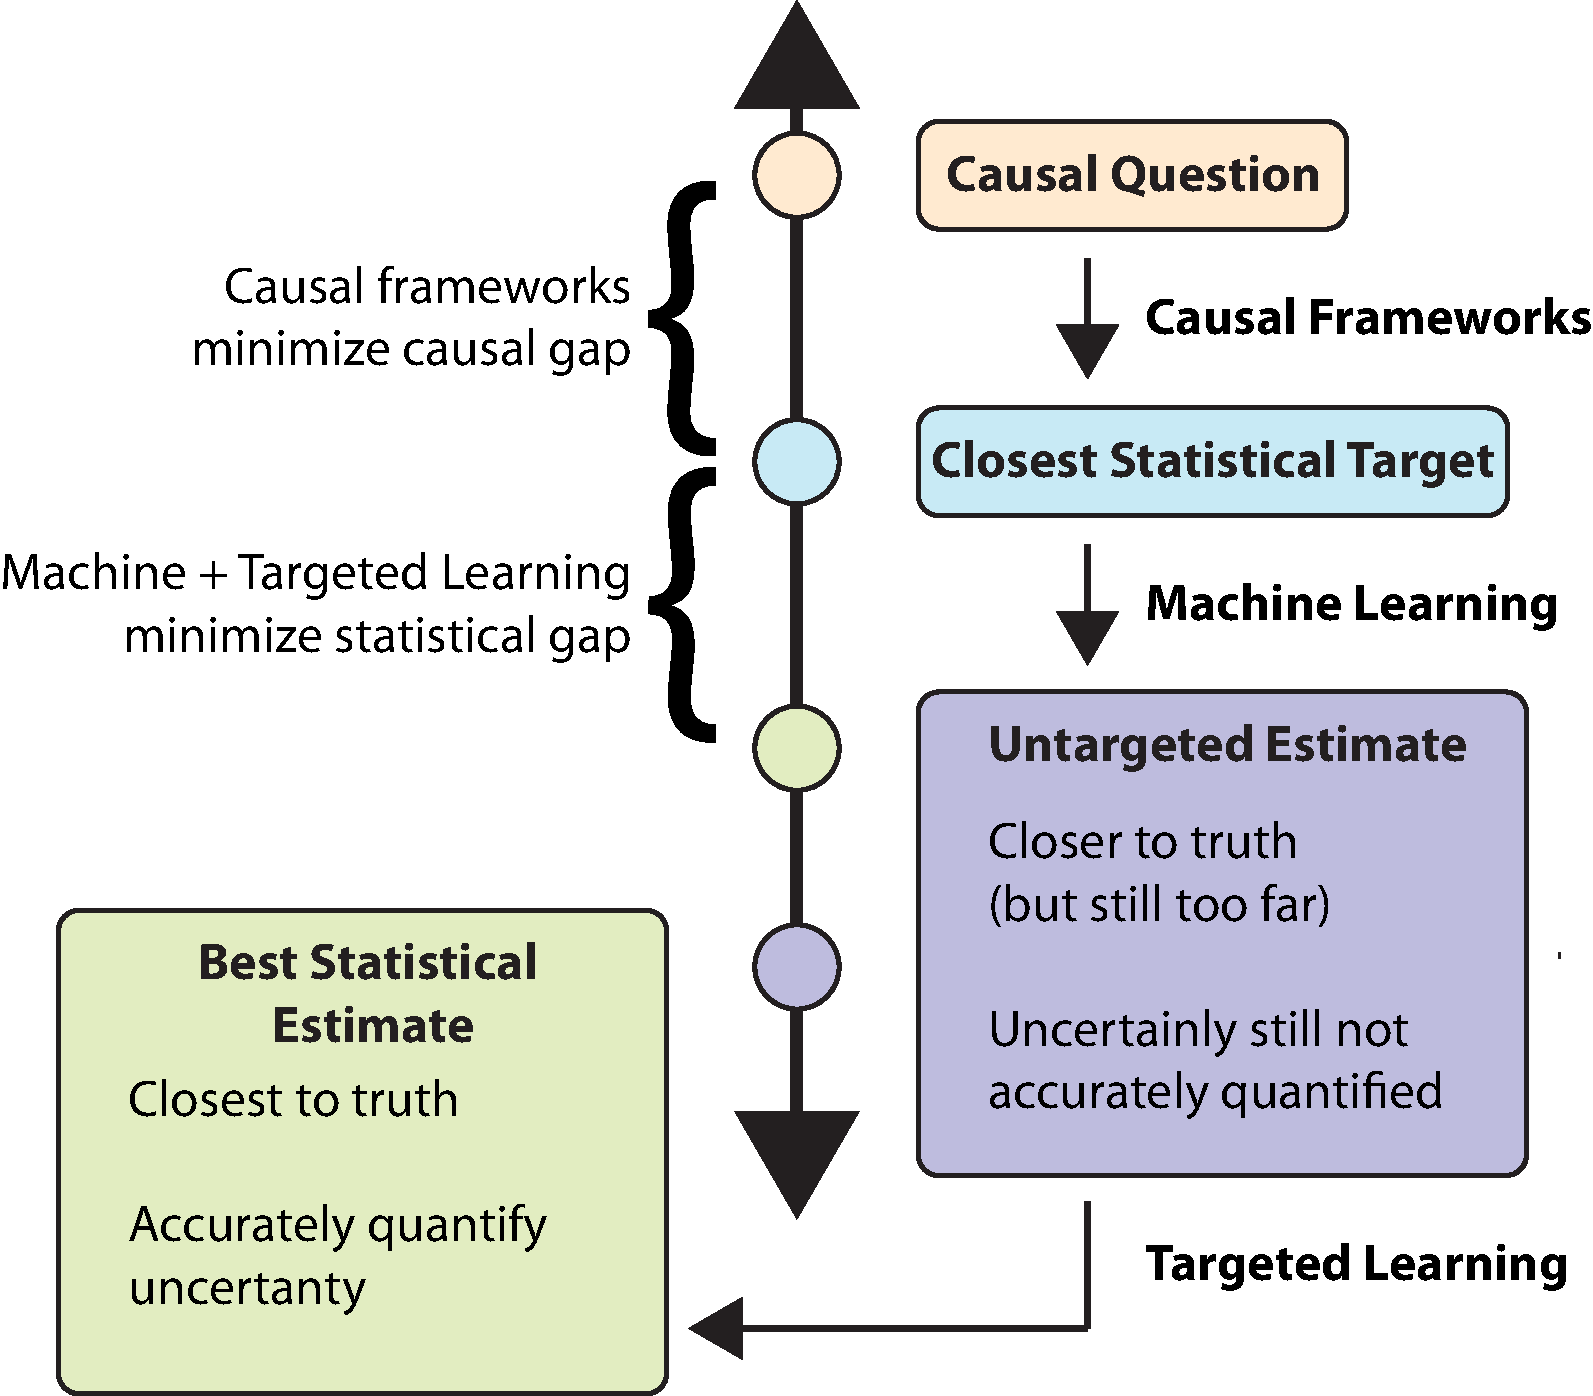
\includegraphics[width=.84\textwidth]{schematic.pdf} \end{center}\end{frame}
%\begin{frame}\frametitle{Targeted Learning is a subfield of statistics}\vspace{-25pt}\begin{columns}\begin{column}{4.9cm}\begin{center}\begin{figure}\fbox{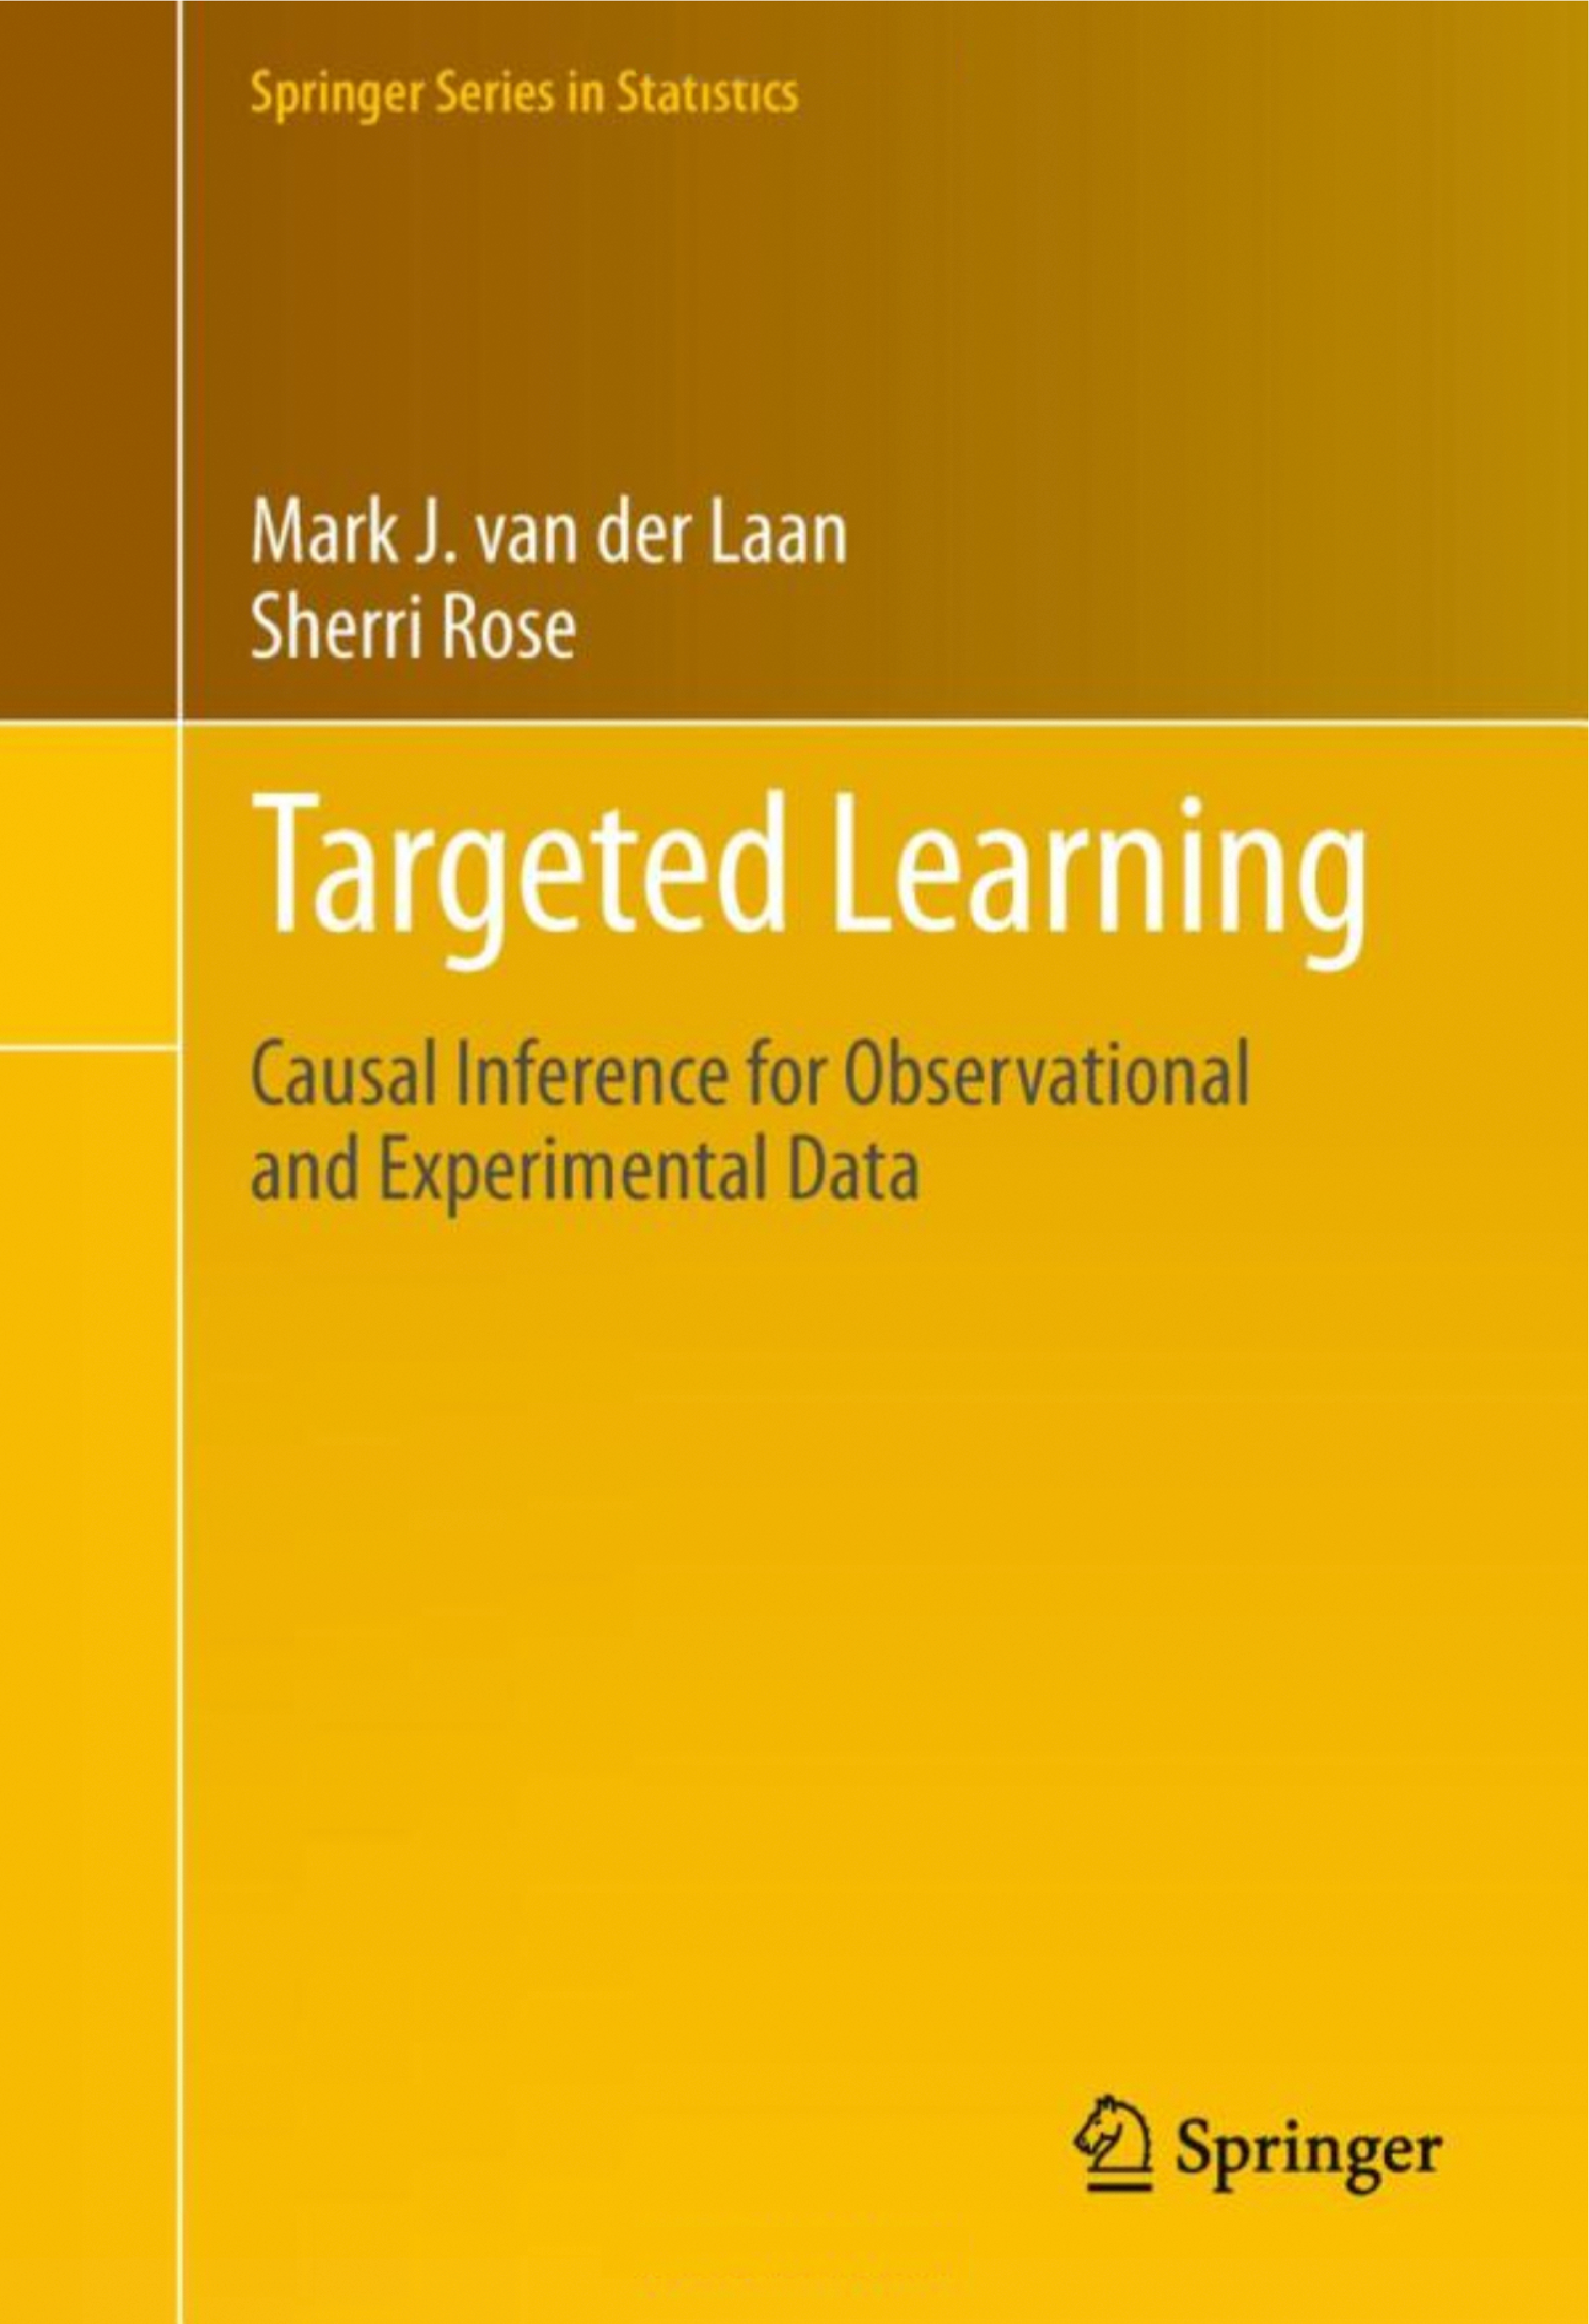
\includegraphics[height=1.7in]{2011Book.pdf}}\end{figure}\end{center}\end{column}\begin{column}{4.9cm}\begin{figure}\fbox{\includegraphics[height=1.7in]{2018Book.pdf}}\end{figure}\end{column}\end{columns}\vspace{-10pt}\begin{columns}\begin{column}{4.9cm}\begin{center}{\footnotesize van der Laan \& Rose, \textit{Targeted Learning: Causal Inference for Observational and Experimental Data}. New York: Springer, 2011.}\end{center}\end{column}\begin{column}{4.9cm}\begin{center}{\footnotesize van der Laan \& Rose, \textit{Targeted Learning in Data Science: Causal Inference for Complex Longitudinal Studies}. New York: Springer, 2018.}\end{center}\end{column}\end{columns}\vspace{15pt}\centering
% \href{https://vanderlaan-lab.org}{https://vanderlaan-lab.org} \hspace{10mm} \href{https://tlverse.org/tlverse-handbook/}{The Hitchhiker’s Guide to the \texttt{tlverse}}\end{frame}





%The challenge facing modern statisticians (and you, as students in this %class) is how to develop statistical methods aimed at answering specific %scientific questions of interest, while utilizing state-of-the-art %algorithms.

%\begin{frame}\frametitle{Targeted Learning is a subfield of statistics}\vspace{-25pt}\begin{columns}\begin{column}{4.9cm}\begin{center}\begin{figure}\fbox{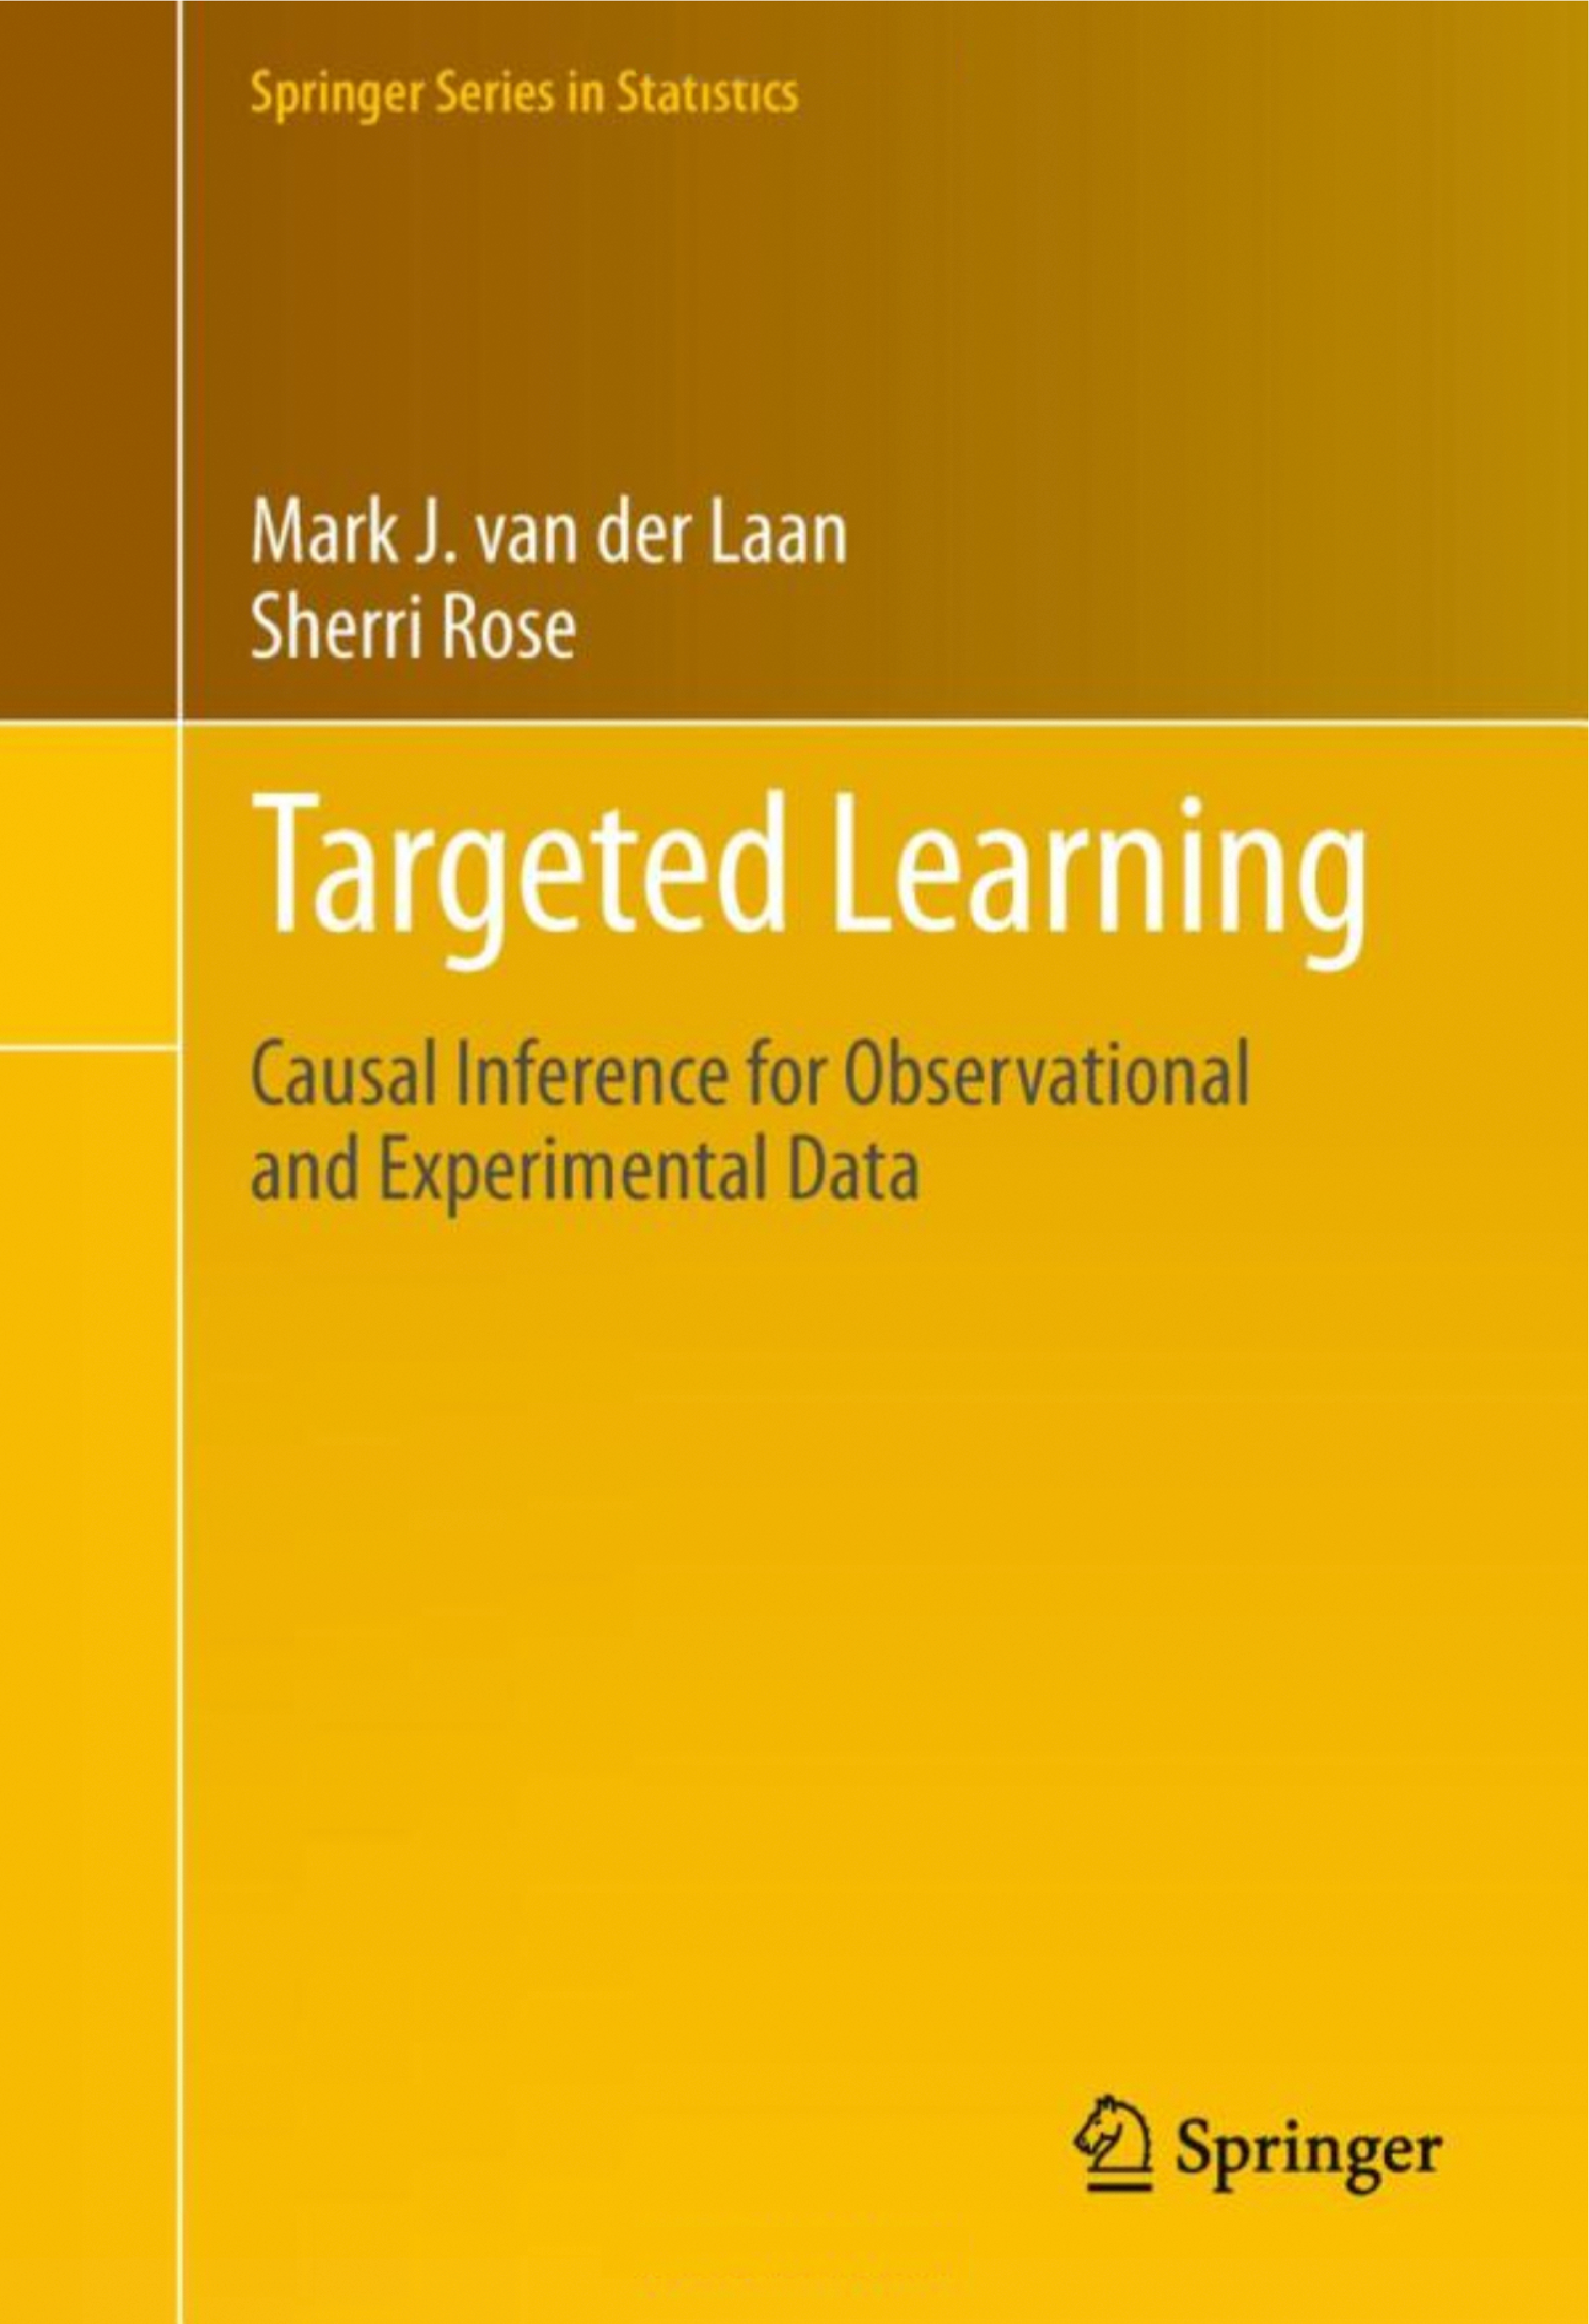
\includegraphics[height=1.7in]{2011Book.pdf}}\end{figure}\end{center}\end{column}\begin{column}{4.9cm}\begin{figure}\fbox{\includegraphics[height=1.7in]{2018Book.pdf}}\end{figure}\end{column}\end{columns}\vspace{-10pt}\begin{columns}\begin{column}{4.9cm}\begin{center}{\footnotesize van der Laan \& Rose, \textit{Targeted Learning: Causal Inference for Observational and Experimental Data}. New York: Springer, 2011.}\end{center}\end{column}\begin{column}{4.9cm}\begin{center}{\footnotesize van der Laan \& Rose, \textit{Targeted Learning in Data Science: Causal Inference for Complex Longitudinal Studies}. New York: Springer, 2018.}\end{center}\end{column}\end{columns}\vspace{15pt}\centering
% \href{https://vanderlaan-lab.org}{https://vanderlaan-lab.org} \hspace{10mm} \href{https://tlverse.org/tlverse-handbook/}{The Hitchhiker’s Guide to the \texttt{tlverse}}\end{frame}\begin{frame}\frametitle{Better clinical decisions from observational data}\vspace{-20pt}\begin{center}  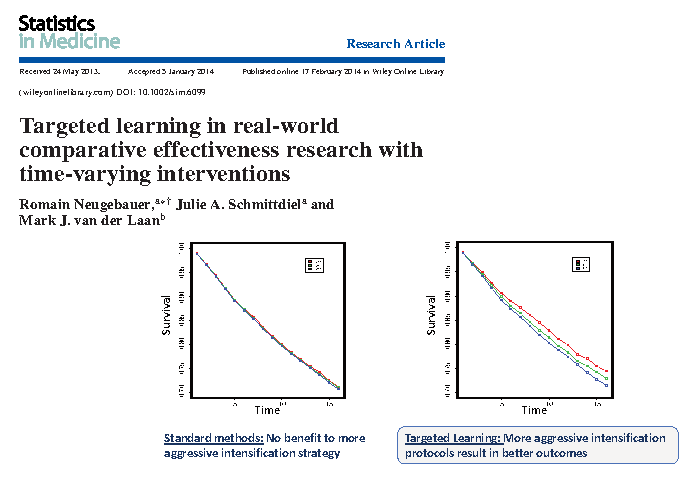
\includegraphics[width = 1.02\textwidth]{diabetes.pdf}  \end{center}\end{frame}



%\section{Statistical Challenges with RWD}

\begin{frame}
\frametitle{Statistical challenges with RWD}
\vspace{20pt}
\begin{center}
\includegraphics[width=\textwidth]{figures/john_slide8_figure.png}
\end{center}
\vspace{35pt}
\tiny{Courtesy of "FDA Real-World Evidence Program" Webinar by John Concato on 4 August 2021}
\end{frame}

\begin{frame}
\frametitle{Statistical challenges with RWD}
\vspace{-18pt}
\begin{center}
\includegraphics[width=1.02\textwidth]{figures/TLpath1_edit.pdf}
\end{center}
\end{frame}

\section{Roadmap TL}

\begin{frame}
  \frametitle{The (causal) roadmap for learning from data}
  \vspace{-20pt}
  \begin{center}
  \includegraphics[width = 1.05\textwidth]{figures/roadmap.pdf}
  \end{center}
\end{frame}

%\subsection{Describe experiment/study}
\begin{frame}
  \frametitle{What is the experiment that generated the data?}
  \vspace{-20pt}
  \begin{center}
  \includegraphics[width = 1.05\textwidth]{figures/roadmap1_1.pdf}
  \end{center}
\end{frame}

\begin{frame}
  \frametitle{What is the experiment that generated the data?}
  \vspace{-20pt}
  \begin{center}
  \includegraphics[width = 1.05\textwidth]{figures/roadmap1_2.pdf}
  \end{center}
\end{frame}


%\subsection{Specify realistic statistical model}
\begin{frame}
  \frametitle{What is known about stochastic relations of the observed variables?}
  \vspace{-20pt}
  \begin{center}
  \includegraphics[width = 1.05\textwidth]{figures/roadmap2.pdf}
  \end{center}
\end{frame}

\begin{frame}
\frametitle{What happens when the statistical model is misspecified and does not contain the DGP?}
\vspace{15pt}
\centering
\includegraphics[width=1.05\textwidth]{figures/misspecified.pdf}
\end{frame}

%\subsection{Define statistical estimand}
\begin{frame}
  \frametitle{Step 3a: What is the target causal estimand that we aim to identify from the data?}
  % defining full-data
  \vspace{-20pt}
  \begin{center}
  \includegraphics[width = 1.05\textwidth]{figures/roadmap3_1.pdf}
  \end{center}
\end{frame}

\begin{frame}
  \frametitle{Step 3b: What is the target statistical estimand? Possibly circle back when lack of power}
 \vspace{-20pt}
 % \vspace{-30pt}
  \begin{center}
  \includegraphics[width = 1.05\textwidth]{figures/roadmap3_2.pdf}
  \end{center}
\end{frame}

%\subsection{Construct estimator}
\begin{frame}
  \frametitle{How should we estimate the target estimand?}
  \vspace{-20pt}
  \begin{center}
  \includegraphics[width = 1.05\textwidth]{figures/roadmap4.pdf}
  \end{center}
\end{frame}

\begin{frame}
  \frametitle{Targeted Maximum Likelihood Estimation (TMLE)}
  \vspace{-20pt}
  \begin{center}
  \includegraphics[width = 1.05\textwidth]{figures/roadmap4_1.pdf}
  \end{center}
\end{frame}

\section{TMLE/SL/HAL}
\begin{frame}
\frametitle{TMLE Step 1: Super learner}
\vspace{-15pt}
\begin{center}
\includegraphics[width = 1\textwidth]{figures/SL.pdf}
\end{center}
\end{frame}
\begin{frame}
\frametitle{Zero-order Highly Adaptive Lasso (HAL): A nonparametric MLE}

\begin{block}{\large{Key Idea}}
\begin{itemize}
\vspace{.1in}
\item Any $d$-dimensional cadlag function (i.e.~right-continuous) can be represented as an infinite linear combination of spline basis functions.
\vspace{.05in}
\item The variation norm / complexity of a function is the $L_1$-norm of the vector of coefficients.
\vspace{.1in}
\end{itemize}
\end{block}

\vspace{.25in}

\begin{center}
{\large Zero-order HAL converges to true function at rate $n^{-1/3}(\log n)^{d/2}$ (only assuming finite variation norm!)}
\end{center}

\end{frame}

\begin{frame}
\frametitle{Zero-order HAL performance for d=3}
  \vspace{-10pt}
  \begin{center}
  \includegraphics[width = 1\textwidth]{HALworks.png}
  \end{center}
\end{frame}

\begin{frame}{New Results: Asymptotic normality of higher order HAL-MLE itself, van der Laan, 2023}
\begin{itemize}
\item Defined higher order smoothness classes $D^{(k)}_C([0,1]^d)$ with global complexity measure $C$, $k=0,\ldots$.
\item We define MLE over this model ($k$-th order HAL).
\item $D^{(k)}_C([0,1]^d)$ can be represented as linear span of tensor products of $\leq k$-th order spline basis functions, where  $L_1$-norm is bounded by $C$.
\item So implementation can be carried out with glmnet().
\item With $J$ basis functions, one obtains uniform approximation error $O(1/J^{k^*})$ up till $\log J$-factor, $k^*=k+1$.
 \item HAL-MLE $Q_n=\sum_{j\in {\cal R}_n}\beta_n(j)\phi_j$ with $J_n$  non-zero coefficients of its oracle MLE  $Q_{0,n}=\sum_{j\in {\cal R}_n}\beta_{0,n}(j)\phi_j$ satisfies $(J_n/n)^{1/2}(Q_n-Q_{0,n})(x)\Rightarrow_d N(0,\sigma^2_0(x))$, while $|| Q_{0,n}-Q_0 ||_{\infty}\sim O(1/J_n^{k^*})$. 
\item By selecting $J_n\sim n^{1/(k^*+1)}$, rate equals $n^{-k^*/(2k^*+1)}$ up till $\log n$-factors. HAL will do this for you.
\end{itemize}
\end{frame}
\begin{frame}{New Results on higher order HAL-MLE}
\begin{itemize}
\item So first order HAL converges at rate $n^{-2/5}$ pointwise, ignoring $\log n$-factors. 
\item At cost of another $\log n$-factor this rate is uniform in $x$. 
\item Pointwise and simultaneous  confidence intervals follow.
\item Any of these HAL-estimators result in plug-in estimators of smooth target features that converge at $n^{-1/2}$ and are asymptotically normal, and either efficient and super-efficient (on set of measure zero!).
\item Inference can be based on nonparametric bootstrap.
\end{itemize}

\end{frame}

\begin{frame}
\frametitle{TMLE Step 2: Targeting follows a path of maximal change in target estimand per unit likelihood}
\vspace{-12pt}
\centering
\begin{figure}
\centering
\animategraphics[autoplay,loop,width=0.95\linewidth]{7}{ULFS_n400/gganim_plot}{0001}{0100}
\end{figure}
\end{frame}


%\subsection{Obtain inference}
\begin{frame}
  \frametitle{Fast approximation of sampling distribution of TMLE?}
  \vspace{-20pt}
  \begin{center}
  \includegraphics[width = 1.05\textwidth]{figures/roadmap5.pdf}
  \end{center}
\end{frame}

%\begin{frame}\frametitle{Can we break HAL-TMLE?}\vspace{-15pt}\begin{center}\includegraphics[width = 1\textwidth]{coverageByN.pdf}\end{center}\end{frame}


%\begin{frame} \frametitle{Possibility to refine question of interest and inform future studies}  \vspace{-11pt}  \begin{center}  \includegraphics[width = 1.0\textwidth]{figures/roadmap_alt1.pdf}\end{center}\end{frame}

%\subsection{Make substantive conclusion}

\begin{frame}
\frametitle{Arriving at the substantive conclusion}
\vspace{-16pt}
  \begin{center}
  \includegraphics[width = 1.02\textwidth]{figures/roadmap6.pdf}
  \end{center}
\end{frame}

\begin{frame}
\frametitle{TL-based non-parametric sensitivity analysis
RCT with 25\% LTFU example}
\vspace{-10pt}
  \begin{center}
  \includegraphics[width = 1.05\textwidth]{figures/gruber_sensitivity.png}
  \end{center}
  \vspace{35pt}
\tiny{Courtesy of "Targeted-Learning Based Statistical Analysis Plan" Webinar by Susan Gruber on 28 April 2021}
\end{frame}

%\begin{frame}\frametitle{TL-based non-parametric sensitivity analysis:Safety analysis example}\vspace{-18pt}  \begin{center}\includegraphics[width = 1.01\textwidth]{figures/sens_plot.pdf}  \end{center}\end{frame}


%\section{Targeted Learning with RWD}



\section{Specification TMLE}

%\begin{frame}{FDA Funded Demonstration Project}FDA has funded a two year demonstration project of TL (led by Susan Gruber) involving \begin{itemize}\item Simulations imitating real world studies demonstrating the roadmap and showcasing that TMLE outperforms propensity score matching and  other current methods of choice.\item Weekly meetings with senior FDA statisticians and us (S. Gruber, Rachael Philips, MvdL).\item Monthly meetings updating the leadership of real world analytics group at FDA.\item Workshop on TL at FDA\item Publications of various articles reporting on findings.\item Regular seminars on topics in TL, recorded and  made public.\item Educational short videos on key concepts in TL.\end{itemize}\end{frame}



%\begin{frame}{FDA funded Sentinel Innovation Center on Causal inference with Real World Data}\begin{itemize}\item Sentinel is the FDA national electronic system transforming the way researchers monitor the safety of FDA-regulated medical products. Launched in response to FDA Amendments Act of 2007. \item Innovation Center  is  led by Department of Pharmacoepidemiology  of Harvard University\item Working group includes FDA, Pharma, and academic statisticians. \item One project  is about how to apply TL to real world data sets in Sentinel system, and evaluating its performance relative to other approaches. \end{itemize}\end{frame}\begin{frame}{Using Innovation Center to showcase how to set up TL Statistical Analysis Plan (SAP) }\begin{itemize}\item Specification of a TMLE relies on various choices that can be tailored towards precise application in questione.g., library of super-learner; truncation method; collaborative  TMLE or not. \item Outcome blind version of data set in question to set  up simulation of (similar) data sets for which we know the truth.\item Select a TMLE optimizing power while controlling type-I error and coverage. \item Results demonstrate for particular rare outcome diseases that C-TMLE is superior thereby providing the choice of SAP, which will then be applied to real data.\item Publication: R. Wyss et al. (2023). Targeted Learning with the Collaborative Controlled Lasso for Large-Scale Covariate Adjustment in Healthcare Database Studies. (under review)\end{itemize}\end{frame}

\begin{frame}\frametitle{Outcome blind simulations to a priori define TMLE: Wyss et al., 2023}


\centering
\begin{figure}
\begin{center}
\includegraphics[width=1.02\textwidth]{abbviepdfslides_2.pdf}
\end{center}
\end{figure}
%\vspace{35pt}
{\small R. Wyss et al. (2023). Targeted Learning with the Collaborative Controlled Lasso for Large-Scale Covariate Adjustment in Healthcare Database Studies}



\end{frame}

\begin{frame}
\centering
\begin{figure}
\begin{center}
\includegraphics[width=1.02\textwidth]{abbviepdfslides_3.pdf}
\end{center}
\end{figure}
%\vspace{35pt}
\end{frame}

%\begin{frame}\centering\begin{figure}\begin{center}\includegraphics[width=1.02\textwidth]{abbviepdfslides_4.pdf}\end{center}\end{figure}
%\vspace{35pt}\end{frame}\begin{frame}\centering\begin{figure}\begin{center}\includegraphics[width=1.02\textwidth]{abbviepdfslides_5.pdf}\end{center}\end{figure}%\vspace{35pt}\end{frame}
\begin{frame}
\centering
\begin{figure}
\begin{center}
\includegraphics[width=1.02\textwidth]{abbviepdfslides_6.pdf}
\end{center}
\end{figure}
%\vspace{35pt}
\end{frame}
\begin{frame}
\centering
\begin{figure}
\begin{center}
\includegraphics[width=1.02\textwidth]{abbviepdfslides_7.pdf}
\end{center}
\end{figure}
%\vspace{35pt}
\end{frame}
\begin{frame}
\centering
\begin{figure}
\begin{center}
\includegraphics[width=1.02\textwidth]{abbviepdfslides_8.pdf}
\end{center}
\end{figure}
%\vspace{35pt}
\end{frame}

\begin{frame}
\frametitle{Targeted Learning with RWD}
\vspace{-18pt}
\centering
\begin{figure}
\begin{center}
\includegraphics[width=1.02\textwidth]{figures/TLpath2_edit.pdf}
\end{center}
\end{figure}
\vspace{35pt}
\end{frame}



%\section{Adaptive Designs}

%\begin{frame}\frametitle{Robust inference for adaptive sequential RCTs}\vspace{-15pt}\centering  \includegraphics[scale=0.35]{learnasyougo_cropped.pdf}\end{frame}


% \begin{frame}
% \frametitle{Adapting the randomization probabilities in a sequence of Sepsis RCTs}
% \begin{itemize}
%     \item We sequentially draw 8 blocks of 100 observations $(W_i,A_i,Y_i)$, $W$ including adrenal insufficiency (binary); serum levels.
%     \item At each block, we use {\bf super learning of optimal rule} and TMLE to estimate its {\bf counterfactual death rate}. 
%   % \item For the adaptive design we then set the randomization probabilities for next block accordingly, while balanced design keeps flipping coin when assigning treatment.
%     \item We report performance of the fixed balanced design and the adaptive design learning the optimal rule w.r.t.  {\bf percentage receiving optimal rule}; observed {\bf death rate}; {\bf coverage} of confidence  intervals.
%     \end{itemize}
%     \end{frame}

%\begin{frame}\frametitle{Balanced vs. adaptive sequential design}\centering\animategraphics[autoplay,loop,width=0.8\linewidth]{10}{Survival_PercentSamples/gganim_plot}{0001}{0100}\end{frame}

%\begin{frame}\frametitle{Balanced vs. adaptive sequential design}\vspace{-5pt}\begin{figure}%    \centering    \subfloat{{\animategraphics[autoplay,loop,width=0.49\linewidth,height=0.49\linewidth]{10}{Survival_WidthCI/gganim_plot}{0001}{0100} }}    \subfloat{{\animategraphics[autoplay,loop,width=0.49\linewidth,height=0.49\linewidth]{10}{Survival_MeanOutcome/gganim_plot}{0001}{0100} }}\end{figure}\end{frame}


%\begin{frame}\frametitle{Ongoing Topics in Targeted Learning}\begin{itemize} \item Causal inference with survival and competing risk time to event outcomes (Rijtgaard et al.). \item Sequential adaptive RCTs   \item Online learning. \item Federated Targeted Learning    \item Causal inference for networks: When one person treatment affects another person's outcome   \item Causal inference for time series (e.g., RCT within a single individual).   
  %\item Learning from EHR data with  better confounder control (incorporating NLP).\item Causal inference in continuous time (Rijtgaard et al.).\end{itemize}\end{frame}

%\begin{frame}\frametitle{Robust inference for adaptive sequential RCTs}\vspace{-15pt}\centering  \includegraphics[scale=0.35]{learnasyougo_cropped.pdf}\end{frame}


% \begin{frame}
% \frametitle{Adapting the randomization probabilities in a sequence of Sepsis RCTs}
% \begin{itemize}
%     \item We sequentially draw 8 blocks of 100 observations $(W_i,A_i,Y_i)$, $W$ including adrenal insufficiency (binary); serum levels.
%     \item At each block, we use {\bf super learning of optimal rule} and TMLE to estimate its {\bf counterfactual death rate}. 
%   % \item For the adaptive design we then set the randomization probabilities for next block accordingly, while balanced design keeps flipping coin when assigning treatment.
%     \item We report performance of the fixed balanced design and the adaptive design learning the optimal rule w.r.t.  {\bf percentage receiving optimal rule}; observed {\bf death rate}; {\bf coverage} of confidence  intervals.
%     \end{itemize}
%     \end{frame}

%\begin{frame}\frametitle{Balanced vs. adaptive sequential design}\centering\animategraphics[autoplay,loop,width=0.8\linewidth]{10}{Survival_PercentSamples/gganim_plot}{0001}{0100}\end{frame}

%\begin{frame}\frametitle{Balanced vs. adaptive sequential design}\vspace{-5pt}\begin{figure}%    \centering
    %\caption{Width of the Confidence Interval and Percent Death in Balanced and Adaptive Sequential Trial}%   \subfloat{{\animategraphics[autoplay,loop,width=0.49\linewidth,height=0.49\linewidth]{10}{Survival_WidthCI/gganim_plot}{0001}{0100} }}%
    %\qquad    \subfloat{{\animategraphics[autoplay,loop,width=0.49\linewidth,height=0.49\linewidth]{10}{Survival_MeanOutcome/gganim_plot}{0001}{0100} }}%
    %\label{fig:example}%\end{figure}\end{frame}


\section{Case Studies  TL}

\begin{frame}
\frametitle{}
\vspace{20pt}
\begin{center}
\includegraphics[width=\textwidth]{slidesfdacommittee/1-FDA RWE Subcommittee.pdf}
\end{center}
\vspace{35pt}
%\tiny{Courtesy of "FDA Real-World Evidence Program" Webinar by John Concato on 4 August 2021}
\end{frame}

\begin{frame}
\frametitle{}
\vspace{20pt}
\begin{center}
\includegraphics[width=\textwidth]{slidesfdacommittee/2-FDA RWE Subcommittee.pdf}
\end{center}
\vspace{35pt}
%\tiny{Courtesy of "FDA Real-World Evidence Program" Webinar by John Concato on 4 August 2021}
\end{frame}







\begin{frame}
\frametitle{}
\vspace{20pt}
\begin{center}
\includegraphics[width=\textwidth]{slidesfdacommittee/3-FDA RWE Subcommittee.pdf}
\end{center}
\vspace{35pt}
%\tiny{Courtesy of "FDA Real-World Evidence Program" Webinar by John Concato on 4 August 2021}
\end{frame}
\begin{frame}
\frametitle{}
\vspace{20pt}
\begin{center}
\includegraphics[width=\textwidth]{slidesfdacommittee/4-FDA RWE Subcommittee.pdf}
\end{center}
\vspace{35pt}
%\tiny{Courtesy of "FDA Real-World Evidence Program" Webinar by John Concato on 4 August 2021}
\end{frame}
\begin{frame}
\frametitle{}
\vspace{20pt}
\begin{center}
\includegraphics[width=\textwidth]{slidesfdacommittee/5-FDA RWE Subcommittee.pdf}
\end{center}
\vspace{35pt}
%\tiny{Courtesy of "FDA Real-World Evidence Program" Webinar by John Concato on 4 August 2021}
\end{frame}
\begin{frame}
\frametitle{}
\vspace{20pt}
\begin{center}
\includegraphics[width=\textwidth]{slidesfdacommittee/6-FDA RWE Subcommittee.pdf}
\end{center}
\vspace{35pt}
%\tiny{Courtesy of "FDA Real-World Evidence Program" Webinar by John Concato on 4 August 2021}
\end{frame}
\begin{frame}
\frametitle{}
\vspace{20pt}
\begin{center}
\includegraphics[width=\textwidth]{slidesfdacommittee/7-FDA RWE Subcommittee.pdf}
\end{center}
\vspace{35pt}
%\tiny{Courtesy of "FDA Real-World Evidence Program" Webinar by John Concato on 4 August 2021}
\end{frame}
\begin{frame}
\frametitle{}
\vspace{20pt}
\begin{center}
\includegraphics[width=\textwidth]{slidesfdacommittee/8-FDA RWE Subcommittee.pdf}
\end{center}
\vspace{35pt}
%\tiny{Courtesy of "FDA Real-World Evidence Program" Webinar by John Concato on 4 August 2021}
\end{frame}

\begin{frame}
\frametitle{}
\vspace{20pt}
\begin{center}
\includegraphics[width=\textwidth]{slidesfdacommittee/9-FDA RWE Subcommittee.pdf}
\end{center}
\vspace{35pt}
%\tiny{Courtesy of "FDA Real-World Evidence Program" Webinar by John Concato on 4 August 2021}
\end{frame}
\section{Deep LTMLE}


\begin{frame}\frametitle{Deep LTMLE: Toru Shirakawa, Yi Li, Sky Qiu, vdL}
\begin{itemize}
\item LTMLE (Bang, Robins, 2005, Petersen et al., Gruber, vdL, etc, relies on {\bf sequential regression}.
%hardest regression dominates; have to discretize time, breaks down for too many time points. 
\item Targeted {\bf maximum likelihood} requires estimation of all conditional densities (vdL 2010a,b; Stitelman etal (2011)).
\item Rijtgaard, Gerds, vdL (2023) {\bf combines}  TM-likelihood based estimation of {\bf intensities}  with estimation of a {\bf conditional mean function integrating over time dependent covariates}.
\item Toru et al. Deep LTMLE utilize {\bf transformer architecture for temporal difference learning}, simultaneously modeling and estimating the sequential regressions: \newline
1)  {\em Computationally superior}; 2) continuous time monitoring; 3)  large histories; 4)  TMLE update step uses transformer gradient descent algorithm. 
% again utilizing same gradient descent algorithm to do the updating simultaneously while solving the EIC score equation.
\end{itemize}
\end{frame} 


%\begin{frame}\frametitle{Pre-specified SAP using SL and TMLE for Cluster RCT's}\begin{itemize}\item    SEARCH 1.0: NCT01864603    \item SEARCH-IPT (a.k.a. SPIRIT): NCT03315962 (Kakande, Lancet HIV, 2022)    \item SEARCH-Youth (a.k.a. SATURN): NCT03848728 (Ruel/Mwangwa, Lancet HIV, 2023)  \item SEARCH-Sapphire Phase A: NCT04810650 with 7 pilots (EtOH, mobility, HTN linkage, HTN treatment, OPD, VHT, ANC) all with separate publications/SAPs\item     SEARCH-CAB-LA: NCT05549726    \item SEARCH-Sapphire Phase B: NCT05768763    \item OPAL: NCT05862857 (aim1) + NCT06036238 (aim2)     \item ENHANCED-SPS (jane CRT for VS among women with HIV who are pregnant or post-partum): NCT04122144    INTEGRATED HIV/HTN (jane CRT for integration of HTN care in HIV care):  NCT04624061\item SEARCH-TB: Really Carina's K01 study on incident TB infection\end{itemize}\end{frame}
%\section{How to a-priori specify TMLE?}

%\begin{frame}{FDA Funded Demonstration Project}FDA has funded a two year demonstration project of TL (led by Susan Gruber) involving \begin{itemize}\item Simulations imitating real world studies demonstrating the roadmap and showcasing that TMLE outperforms propensity score matching and  other current methods of choice.\item Weekly meetings with senior FDA statisticians and us (S. Gruber, Rachael Philips, MvdL).\item Monthly meetings updating the leadership of real world analytics group at FDA.\item Workshop on TL at FDA\item Publications of various articles reporting on findings.\item Regular seminars on topics in TL, recorded and  made public.\item Educational short videos on key concepts in TL.\end{itemize}\end{frame}

\section{Conclusion}
\begin{frame}\frametitle{Concluding Remarks}
\begin{itemize}
\item Roadmap for causal inference and Targeted Learning provides systematic principled approach for generating RWE.
\item Integrates all advances in machine learning, statistical theory and causal identification.
\item SL and TMLE can be tailored towards particular estimation problem in pre-specified manner using outcome blind simulations.
\item HAL provides realistic models;  theoretical guarantees, dimension free rates,  and bridges TMLE to inference for non-pathwise differentiable target functions such as conditional treatment effects, dose response curves etc. 
\item Bridges such as Deep LTMLE to deep learning community are crucial. 
\end{itemize}
\end{frame}
\end{document}
\section{TL in longitudinal RW studies}\begin{frame}\frametitle{General Longitudinal Data Structure for Complex Observational Studies}We observe $n$ i.i.d. copies of a longitudinal data structure\[O=(L(0),A(0),\ldots,L(K),A(K),Y=L(K+1)),\]where $A(t)$ denotes a discrete valued {\bf intervention node} whose effect we desire to evaluate,  $L(t)$ is an intermediate covariate and outcome realized in between intervention nodes $A(t-1)$ and $A(t)$, $t=0,\ldots,K$, and $Y$ is a final {\bf outcome} of interest.\ \newline{\bf Survival outcome example:}For example, \begin{eqnarray*}A(t)&=&(A_1(t),A_2(t))\\A_1(t)&=& \mbox{Indicator of being treated at time $t$}\\A_2(t)&=& \mbox{Indicator of being right-censored at time $t$}\\
%\Delta&=&\mbox{Indicator of observing failure}\\
Y(t)&=&\mbox{Indicator of observing a failure by time $t$}\\L(t)&&\mbox{Vector of time-dependent measurements}\\Y(t)&\subset& L(t)\mbox{and  $Y=Y(K+1)$}.\end{eqnarray*}\end{frame}


% \subsection{Targeted learning in complex observational study of diabetes (Neugebauer et al.)}

\begin{frame}{A real-world CER study comparing different rules for treatment intensification for diabetes}\begin{itemize}\item Data extracted from diabetes registries of 7 HMO research network sites: \begin{itemize}\item Kaiser Permanente\item Group Health Cooperative \item HealthPartners\end{itemize}
%\end{frame}
%\begin{frame}
%\begin{itemize}
\item  {\bf Enrollment period:} Jan 1$^{\textrm{st}}$ 2001 to Jun 30$^{\textrm{th}}$ 2009
\item Patients enrolled the first time treatment intensification (TI) was first indicated as long as the benefits and harms of TI were unclear.
\end{itemize}
 {\bf Enrollment criteria:} \\ 
\vspace{-0.2cm}\begin{itemize}
\item past A1c$<7\%$ (glucose level) while on 2+ oral agents or basal insulin 
\item $7\%\leq$ latest A1c $\leq 8.5\%$  (study entry when glycemia was no longer reined in)
\end{itemize}
\end{frame}

\begin{frame}{Longitudinal data}

\begin{itemize}
\item {\bf Follow-up} til the earliest of Jun 30$^{\textrm{th}}$ 2010, death, health plan disenrollment, or the failure date
\item {\bf Failure} defined as onset/progression of albuminuria (a microvascular complication) 
\item {\bf Treatment} is the indicator being on ''treatment intensification'' (TI)
\item $n\approx 51,000$ with a median follow-up of 2.5 years.
\item {\bf Target estimand:} What would survival look like if treatment is intensified when $A1c<x\%$ for various levels $x=7,7.5,8,8.5$?
\end{itemize}
\end{frame}

\begin{frame}
\frametitle{Likelihood and Statistical Model}
The probability density/likelihood $p_0$ of $O$ can be {\bf factorized according to the time-ordering} as 
\begin{eqnarray*}
p_0(O)&=&\prod_{t=0}^{K+1} p_0(L(t)\mid Pa(L(t)) ) \prod_{t=0}^K p_0(A(t)\mid Pa(A(t)) )\\
&\equiv& \prod_{t=0}^{K+1}q_{0,L(t)}(O)\prod_{t=0}^K g_{0,A(t)}(O)\\
&\equiv& q_0g_0,
\end{eqnarray*}
where $Pa(L(t))\equiv (\bar{L}(t-1),\bar{A}(t-1))$ and $Pa(A(t))\equiv (\bar{L}(t),\bar{A}(t-1))$ denote the parents  of $L(t)$ and $A(t)$ in the time-ordered sequence, respectively. 
The $g_0$-factor represents the {\bf intervention mechanism}.\newline
{\bf Statistical Model:}
We make no assumptions on $q_0$, but could make assumptions on $g_0$.
\end{frame}


\begin{frame}
\frametitle{Statistical Target Parameter: $G$-computation Formula for Post-dynamic-Intervention Distribution}
\begin{itemize}
\item $p^{g^*}_0=q_0(o)g^*(o)$ is the {\bf $G$-computation formula for the post-intervention distribution} of $O$ under the stochastic intervention $g^*=\prod_{t=0}^K g^*_{A(t)}(O)$.
\item Under {\bf sequential randomization assumption} (SRA) and a positivity assumption, the post-intevention distribution $p_{g^*}$ of $O$ equals $p_{g^*}$, where post-intervention distribution is defined by the structural equation model in which the equations for the intervention nodes $A(t)$ are replaced by drawing from $g^*_{A(t)}$.
\item {\bf Causal estimand}: $E_{P_{g^*}}Y$, mean outcome of $Y$ under post-intervention distribution, or survival rate if $Y$ is indicator of survival, under  post-intervention $P_{g^*}$.
\item {\bf Target estimand}: $E_{P^{g^*}}Y$, mean outcome of $Y$ under $G$-computation density.
%\itemIn particular, for a dynamic intervention $d=(d_t: t=0,\ldots,K)$ with $d_t(\bar{L}(t),\bar{A}(t-1))$ being the treatment at time $t$, the $G$-computation formula is given by \begin{align*}\label{eqn:Gcomp}p^d_0(l)=\prod_{t=0}^{K+1}q_{0,L(t)}^d(\bar{l}(t)),\end{align*}
%Susan: replace 1 by bar{a}(k-1)where $q_{L(t)}^d(\bar{l}(t))=q_{L(t)}(l(t)\mid \bar{l}(t-1),\bar{A}(t-1)=\bar{d}_{t-1}(\bar{l}(t-1)) )$. \itemLet $L^d=(L(0),L^d(1),\ldots,Y^d=L^d(K+1))$ denote the random variable with probability distribution $P^d$. 
%\item This is the so called $G$-computation formulafor the post-intervention distribution corresponding with the dynamic intervention $d$.
%It is naturally generalized to the post-intervention distribution for stochastic interventions defined by user-supplied choice $g^*$. 
\end{itemize}
\end{frame}

\begin{frame}
\frametitle{Better clinical decisions from observational data}
\vspace{-20pt}
\begin{center}
  \includegraphics[width = 1.02\textwidth]{diabetes.pdf}
  \end{center}
\end{frame}

% \begin{frame}
% \frametitle{Convergence of adaptive randomization probabilities towards optimal rule}
% \vspace{5pt}
% \centering
% \begin{figure}%
% \includegraphics[scale=0.3]{design_convergence}
% \end{figure}
% \end{frame}


% \begin{frame}{TMLE-based statistical inference for performance under current best estimate of rule}
% \vspace{15pt}
%     \includegraphics[scale=0.3]{adaptive_design_inference}
% \end{frame}
% \subsection{Complex Observational Studies}

% \begin{frame}
% \frametitle{Longitudinal data structure}
% We observe $n$ i.i.d. copies of a longitudinal data structure
% \[
% O=(L(0),A(0),\ldots,L(K),A(K),Y=L(K+1)),\]
% where 
% \begin{itemize}
%     \item $A(t)$ denotes a discrete valued {\bf intervention node} whose effect we desire to evaluate
%     \item $L(t)$ is an {\bf intermediate covariate/outcome} realized in between intervention nodes $A(t-1)$ and $A(t)$, $t=0,\ldots,K$
%     \item $Y$ is the {\bf final outcome} of interest
% \end{itemize}    
% \end{frame}
% \begin{frame}
% \frametitle{Survival outcome example}
% \begin{eqnarray*}
% A(t)&=&(A_1(t),A_2(t))\\
% A_1(t)&=& \mbox{Indicator of being treated at time $t$}\\
% A_2(t)&=& \mbox{Indicator of being right-censored at time $t$}\\
% %\Delta&=&\mbox{Indicator of observing failure}\\
% Y(t)&=&\mbox{Indicator of observing a failure by time $t$}\\
% L(t)&=&\mbox{Vector of time-dependent measurements}\\
% Y(t)&\subset& L(t) \mbox{and  $Y=Y(K+1)$}.
% \end{eqnarray*}
% \end{frame}

% \begin{frame}
% \frametitle{Likelihood and statistical model}
% The probability distribution $P_0$ of $O$ can be factorized according to the time-ordering as 
% \begin{eqnarray*}
% p_0(O)&=&\prod_{t=0}^{K+1} p_0(L(t)\mid Pa(L(t)) ) \prod_{t=0}^K p_0(A(t)\mid Pa(A(t)) )\\
% &\equiv& \prod_{t=0}^{K+1}q_{0,L(t)}(O)\prod_{t=0}^K g_{0,A(t)}(O)\\
% &\equiv& q_0g_0,
% \end{eqnarray*}
% {\footnotesize
% where $Pa(L(t))\equiv (\bar{L}(t-1),\bar{A}(t-1))$ and $Pa(A(t))\equiv (\bar{L}(t),\bar{A}(t-1))$ denote the parents of  $L(t)$ and $A(t)$, respectively. 

% The $g_0$-factor represents the intervention mechanism.}

% \vspace{15pt}

% {\bf Statistical Model:}
% We make no assumptions on $q_0$, but could make assumptions on $g_0$.
% \end{frame}

% \begin{frame}
% \frametitle{Target estimand}
% \begin{itemize}
% \item $p^{g^*}_0=q_0(o)g^*(o)$ is the $G$-computation formula for the post-intervention distribution of $O$ under the stochastic intervention $g^*=\prod_{t=0}^K g^*_{A(t)}(O)$.

% \vspace{20pt}

% \item Target estimand $\Psi(P)=E_{P_{g^*}}Y$, i.e.,  mean outcome under $P_{g^*}$. 
% \end{itemize}
% \end{frame}


